\section{Referencia de la Clase Proveedor\-View}
\label{classProveedorView}\index{ProveedorView@{ProveedorView}}
Muestra y administra la ventana con la informaci\'{o}n de un proveedor.  


{\tt \#include $<$provedit.h$>$}

Diagrama de colaboraci\'{o}n para Proveedor\-View:\begin{figure}[H]
\begin{center}
\leavevmode
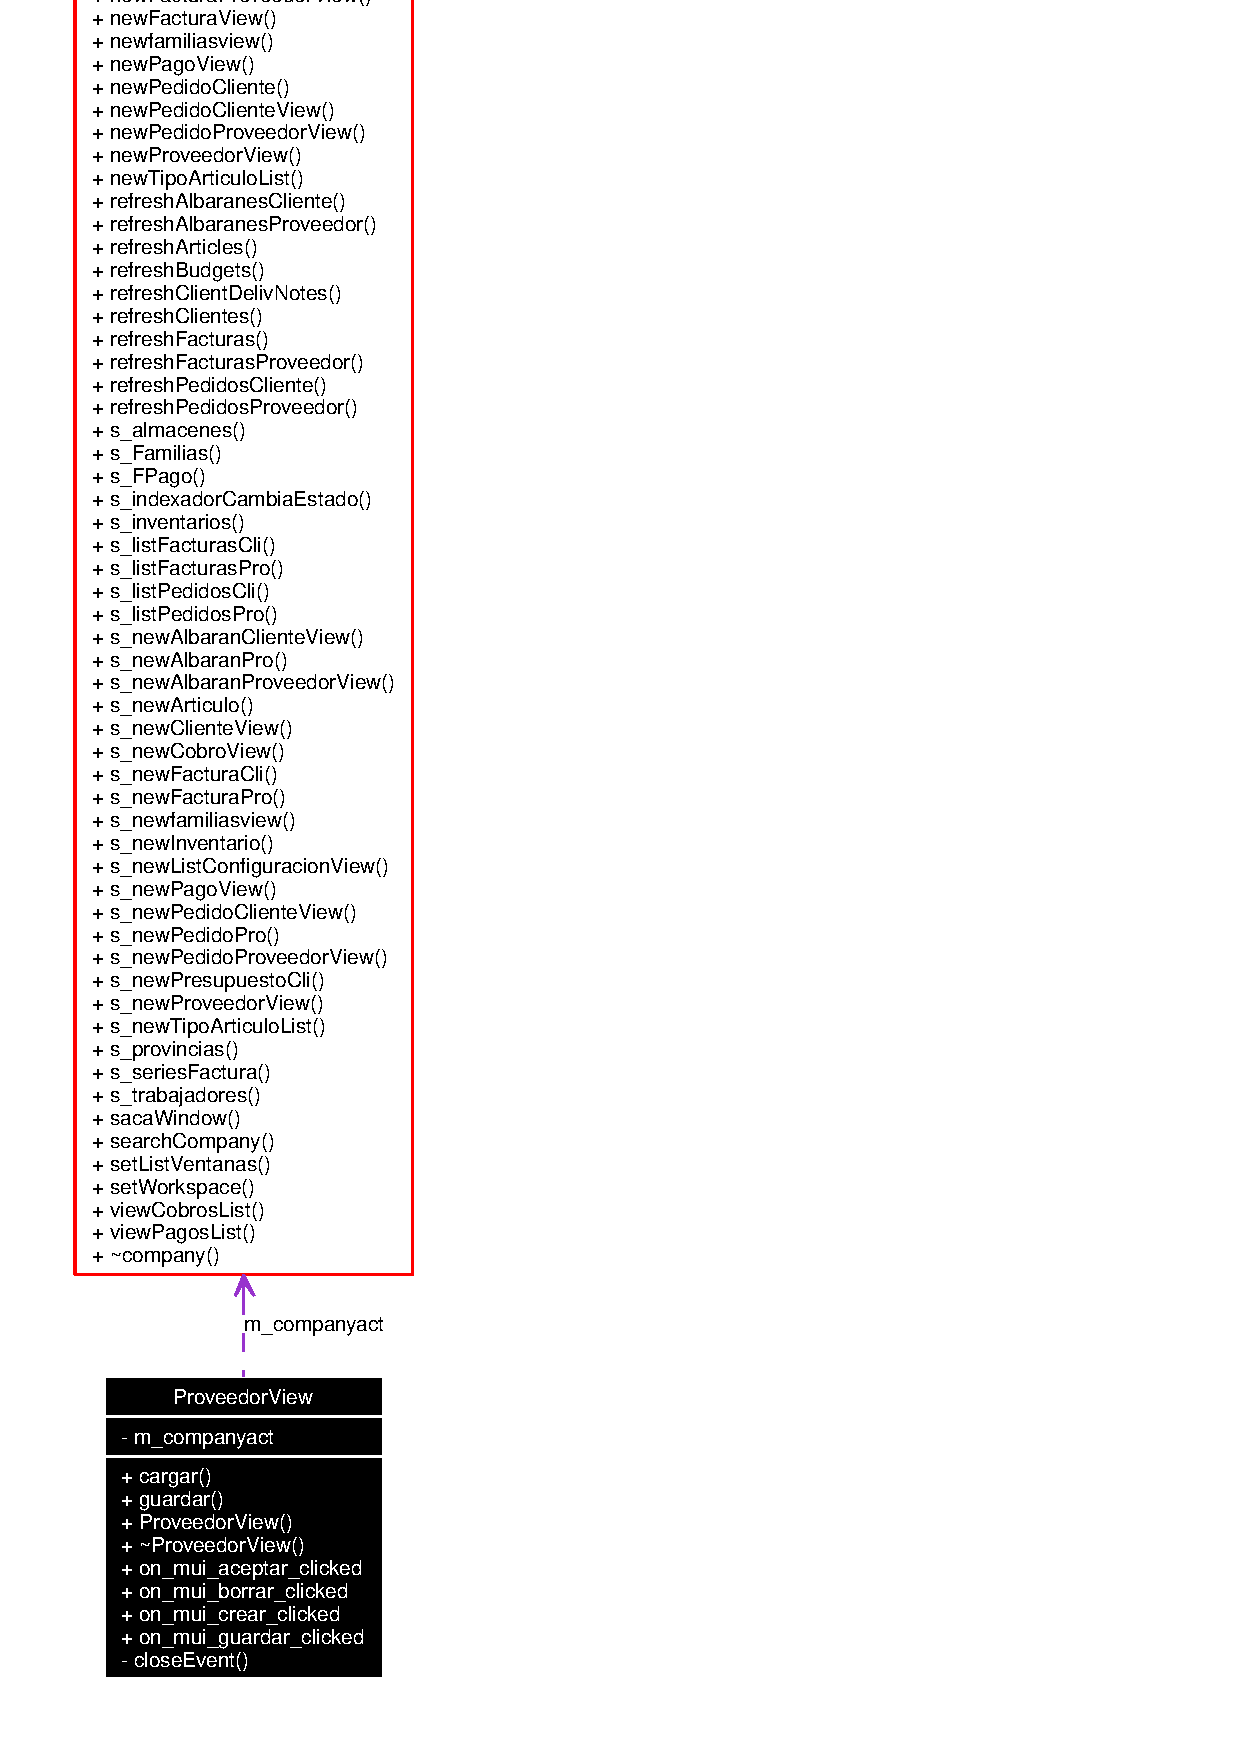
\includegraphics[width=99pt]{classProveedorView__coll__graph}
\end{center}
\end{figure}
\subsection*{Slots p\'{u}blicos}
\begin{CompactItemize}
\item 
virtual void {\bf on\_\-mui\_\-aceptar\_\-clicked} ()\label{classProveedorView_i0}

\item 
virtual void {\bf on\_\-mui\_\-borrar\_\-clicked} ()\label{classProveedorView_i1}

\begin{CompactList}\small\item\em Esta funcion se ejecuta cuando se ha pulsado sobre el boton de borrar. \item\end{CompactList}\item 
virtual void {\bf on\_\-mui\_\-crear\_\-clicked} ()\label{classProveedorView_i2}

\begin{CompactList}\small\item\em Esta funcion se ejecuta cuando se ha pulsado sobre el boton de nuevo. \item\end{CompactList}\item 
virtual void {\bf on\_\-mui\_\-guardar\_\-clicked} ()\label{classProveedorView_i3}

\end{CompactItemize}
\subsection*{M\'{e}todos p\'{u}blicos}
\begin{CompactItemize}
\item 
virtual int {\bf cargar} (QString)
\item 
virtual int {\bf guardar} ()
\item 
{\bf Proveedor\-View} ({\bf company} $\ast$emp, QWidget $\ast$parent=0)
\end{CompactItemize}


\subsection{Descripci\'{o}n detallada}
Muestra y administra la ventana con la informaci\'{o}n de un proveedor. 



\subsection{Documentaci\'{o}n del constructor y destructor}
\index{ProveedorView@{Proveedor\-View}!ProveedorView@{ProveedorView}}
\index{ProveedorView@{ProveedorView}!ProveedorView@{Proveedor\-View}}
\subsubsection{\setlength{\rightskip}{0pt plus 5cm}Proveedor\-View::Proveedor\-View ({\bf company} $\ast$ {\em comp}, QWidget $\ast$ {\em parent} = {\tt 0})}\label{classProveedorView_a2}


Desabilitamos los tabs que aun no se usan

Cargamos el listado de pedidos del proveedor y dejamos presentable. 

\subsection{Documentaci\'{o}n de las funciones miembro}
\index{ProveedorView@{Proveedor\-View}!cargar@{cargar}}
\index{cargar@{cargar}!ProveedorView@{Proveedor\-View}}
\subsubsection{\setlength{\rightskip}{0pt plus 5cm}int Proveedor\-View::cargar (QString {\em idprov})\hspace{0.3cm}{\tt  [virtual]}}\label{classProveedorView_a0}


Esta funcion carga un proveedor de la base de datos y lo presenta. Si el parametro pasado no es un identificador valido entonces se pone la ventana de edicion en modo de insercion.

Cargamos las ventanas auxiliares.

Cambiamos el titulo de la ventana para que salga reflejado donde toca. \index{ProveedorView@{Proveedor\-View}!guardar@{guardar}}
\index{guardar@{guardar}!ProveedorView@{Proveedor\-View}}
\subsubsection{\setlength{\rightskip}{0pt plus 5cm}int Proveedor\-View::guardar ()\hspace{0.3cm}{\tt  [virtual]}}\label{classProveedorView_a1}


Esta funcion es la respuesta a la pulsacion del boton de guardar Comprueba si es una insercion o una modificacion y hace los pasos pertinentes.

Disparamos los plugins con presupuesto\_\-imprimir\-Presupuesto 

La documentaci\'{o}n para esta clase fu\'{e} generada a partir de los siguientes archivos:\begin{CompactItemize}
\item 
provedit.h\item 
provedit.cpp\end{CompactItemize}
